
With a baseline in the thesis' theoretical and methodological groundwork, the following chapter will showcase the main empirical results in relation to the hypotheses. Initially, section \ref{ST_results} examine the short-term investor reactions to negative and positive events. In addition, the overall reactions are complemented by a review of how news related to the specific SDGs are anticipated by investors. Finally, section \ref{sec: long_term_portfolio} explore the long-term abnormal return from reactions to SDG news. To explore whether investors integrate the sustainability level of a company, I assess the investor reactions with a partition on the companies' ESG risk ratings. 

For simplicity, in the context of negative events, I will communicate the abnormal return in absolute values, as it aligns with the assumption of taking a short position in the asset that experiences a negative event. Therefore, a decrease in the AAR on the graphs or the alpha in the tables corresponds to an increase in abnormal returns.


\subsection{Short Term Abnormal Returns} \label{ST_results}
To test hypothesis #1 of whether SDG-related events impact firms' market values in the short term, I separate negative and positive events and assess the development in abnormal returns 10 days before and 10 days after the occurrence of an event. Additionally, I examine whether investor reactions differ depending on the SDG to which the news is related to and the ESG risk of the company.

\subsubsection{Negative News} \label{sec: st_negative}

\textbf{Overall SDGs.} The average abnormal returns (AAR) and development in cumulative average abnormal returns (CAAR) after a negative event is illustrated in figure \ref{fig:ST_neg_news}. The left y-axis represents the abnormal return, while the x-axis displays the number of days before and after an event has occurred. To support the analysis, the graph also includes the 95\% confidence intervals of the AAR and CAAR. Additionally, the white bars in the background represent the number of events on a given day relative to the event day $(t = 0)$, shown on the right axis. 

The AAR (in blue) represents the abnormal return for the average firm on a given day relative to the event. For example, on the date of the event, at $t=0$, the AAR is significantly negative at -0.17\% with a 5\% level of significance. This indicates that investors react to spikes in bad news by selling their shares. In contrast, on the first day of the event window, at $t=-10$, no investor reaction is present, since the AAR is not significantly different from zero. This day, $t=-10$ represents the reaction 10 days before an event for the average firm. Similarly, the CAAR is simply the accumulated value of the AAR across the event window. 

Thus, we can interpret from the graph, that the event itself is not followed by a significant reaction, as the days following an event demonstrates no abnormal performance. Moreover, the investor reaction does not materialize in the initial days of the window, from $t = -10$ to $t = -7$. After this initial period, the AAR start to decrease, which indicates a loss in market share prior to the observed event. The overall reaction is represented through the CAAR, which is significantly negative from $t=-4$ and through the remaining window where it bottoms at approximately $-0.72\%$ 10 days after an event. The declining trend of the CAAR suggests that the market gradually learns about the negative events. Thus, new information appears to be priced in prior to the spike in news articles.


\begin{figure} [H]
    \centering
    \caption{Negative News: AAR and CAAR}
    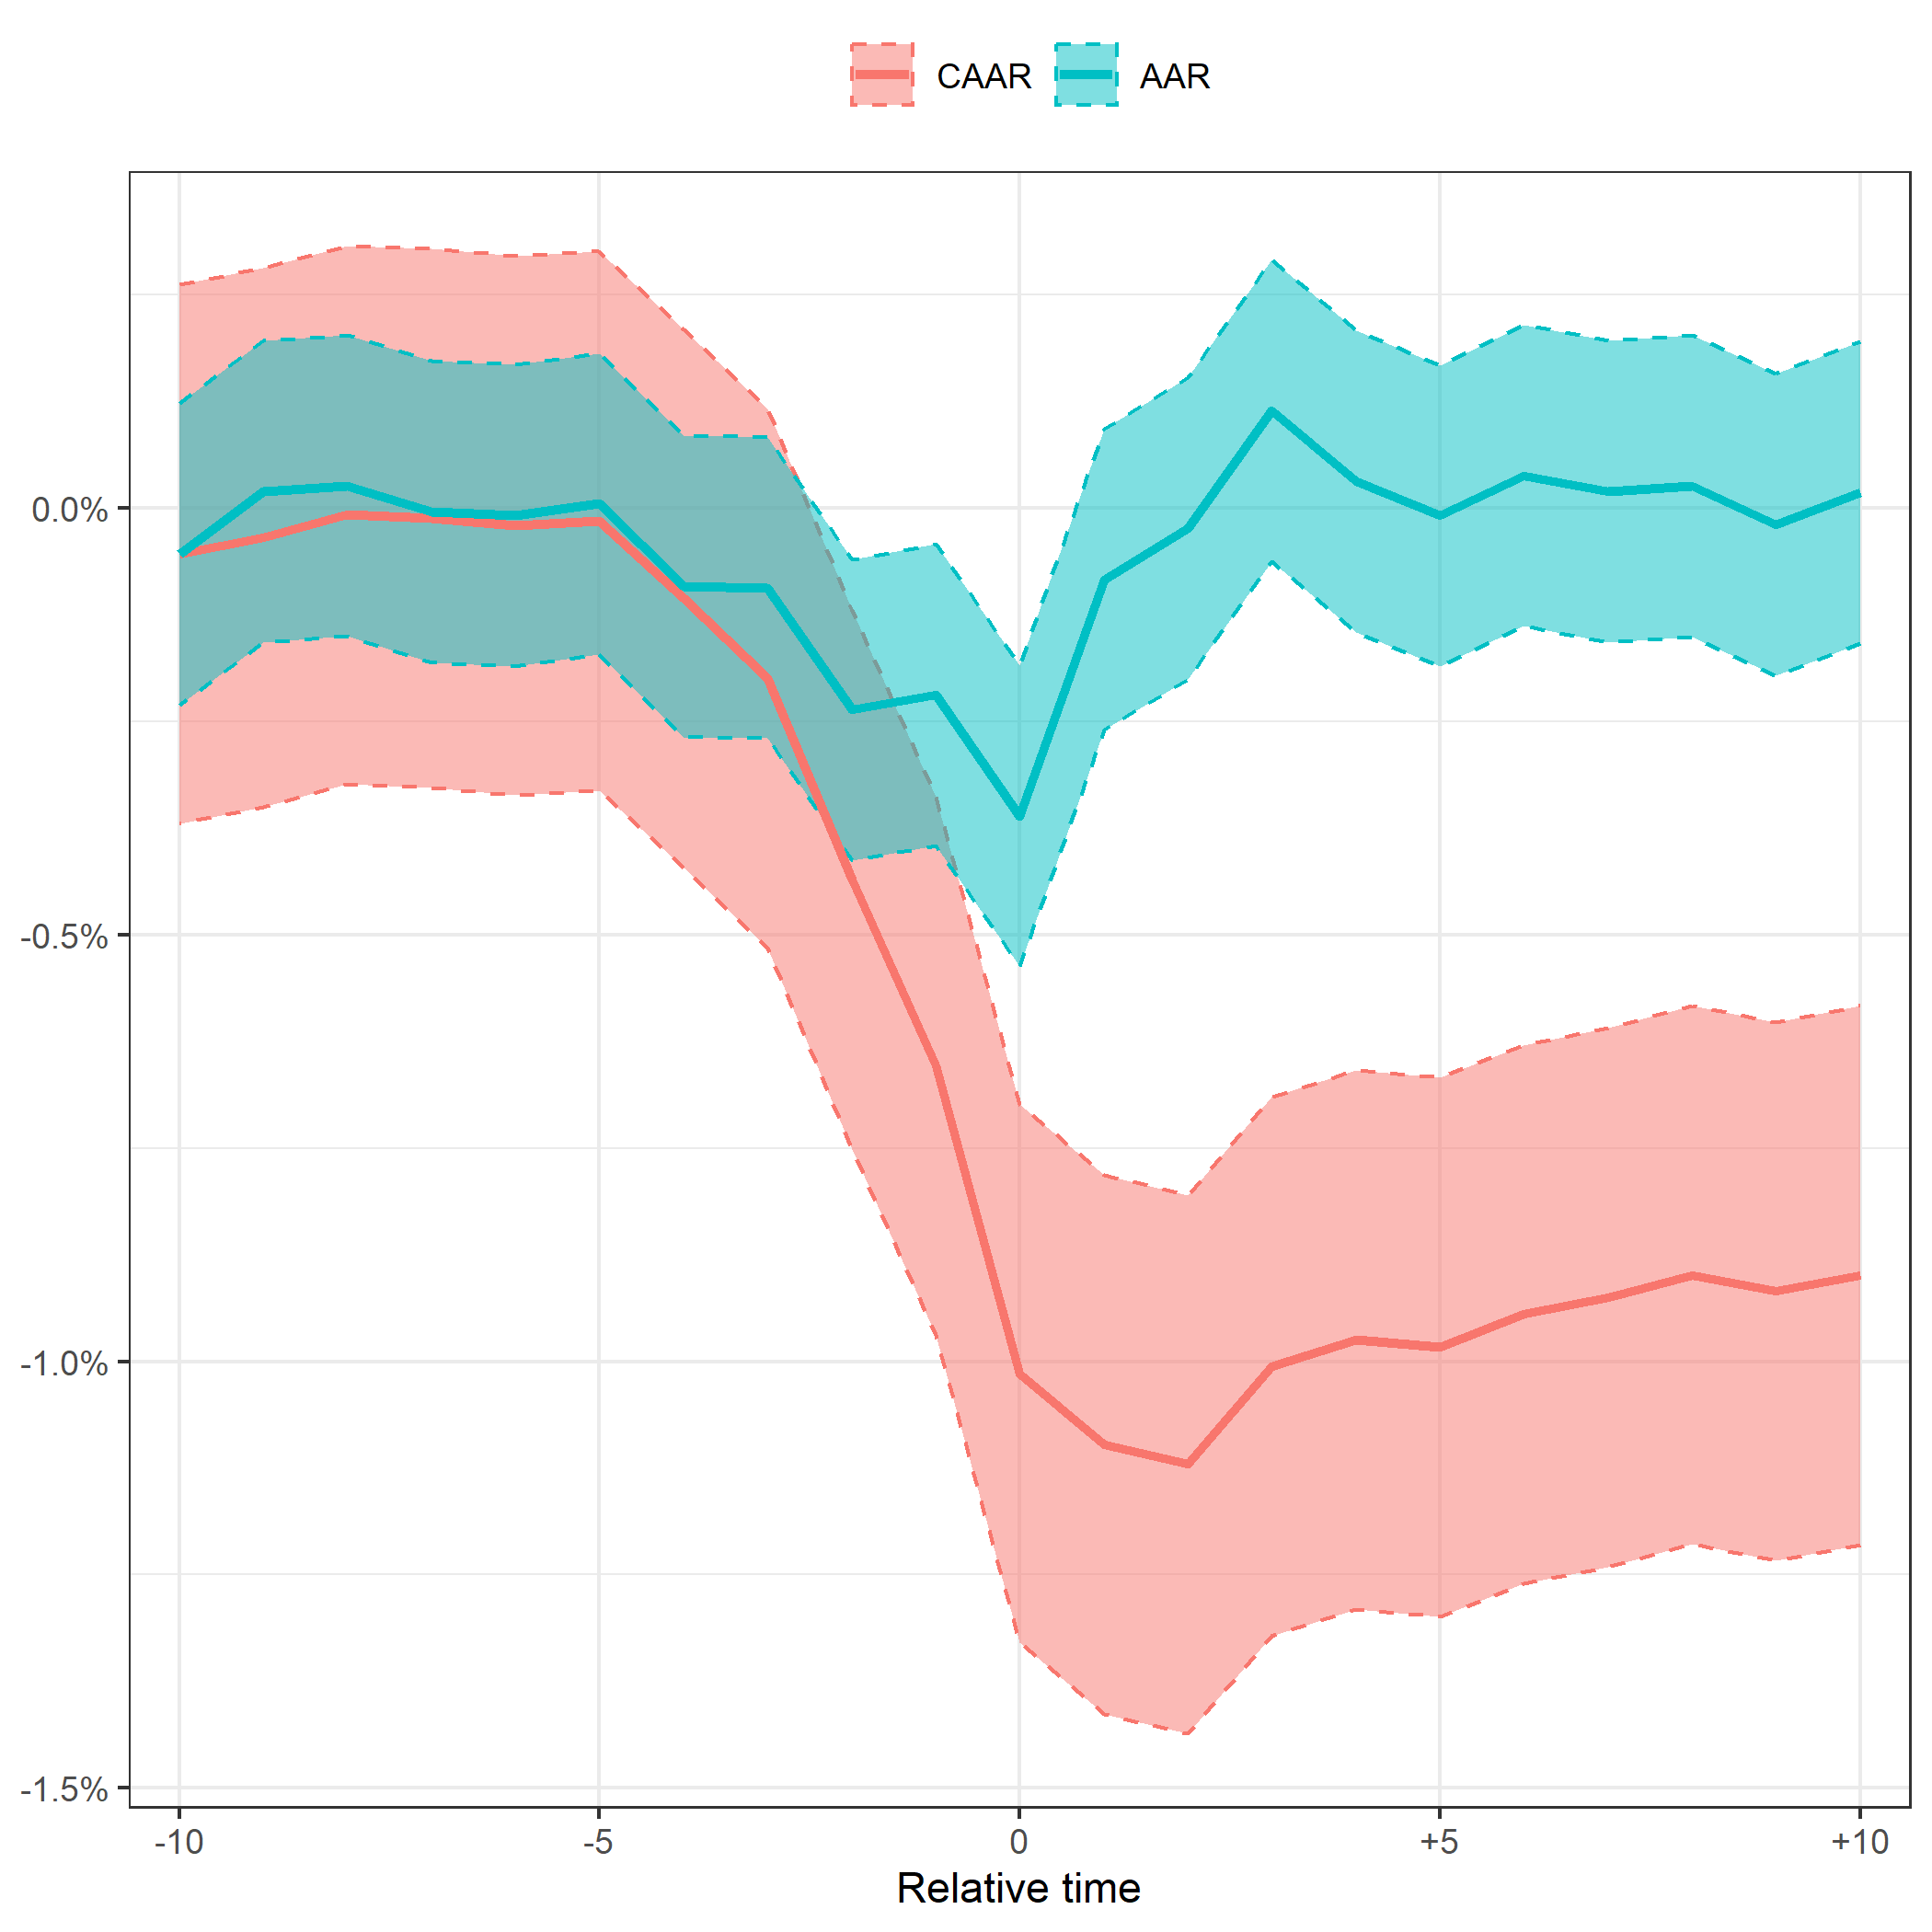
\includegraphics[scale=0.6]{Projekt/1.Figures analysis/ST_negative_all_CI.png}
     \caption*{\footnotesize The figure illustrates the AAR and CAAR around the event date (t = 0) after negative events, along with 95\% confidence intervals and the relative number of events on a given day relative to the event date (rhs). The outcome is based on N = 1618 events. On the date of the average event, $t=0$, investors react by selling the average stock with an AAR of $-0.17\%$. The reaction is similar several days prior to the event is identified. This results in a CAAR of $-0.72\%$ over the entire period.  
      }
    \label{fig:ST_neg_news}
\end{figure} 
 
The bars in the background offer insights into the extent of media attention during the days surrounding a spike in news. For instance, at $t = -1$ the average firm is mentioned in nearly 50\% fewer articles compared to the number of articles on $t = 0$. The bars increase as the CAAR begin to decline, suggesting a relation between media attention towards negative news and pessimistic investor behavior. These results are indicative of an initial relation between negative news and investor reactions. 

\noindent \textbf{Partition on ESG risk.} To further investigate whether the degree of sustainability of firms influence the performance of abnormal returns  after encountering news, I estimate the model with a partition based on company ESG risk ratings. Figure \ref{fig:ST_neg_ESG} follows the same setup as figure \ref{fig:ST_neg_news} and displays the CAAR of event firms with a partition on ESG risk. In this analysis, the "Low" rating indicates that a firm has a low risk of encountering complications in relation to ESG affairs.

\begin{figure} [h]
    \centering
    \caption{CAAR Partitioned on ESG Risk Ratings: Negative News }
    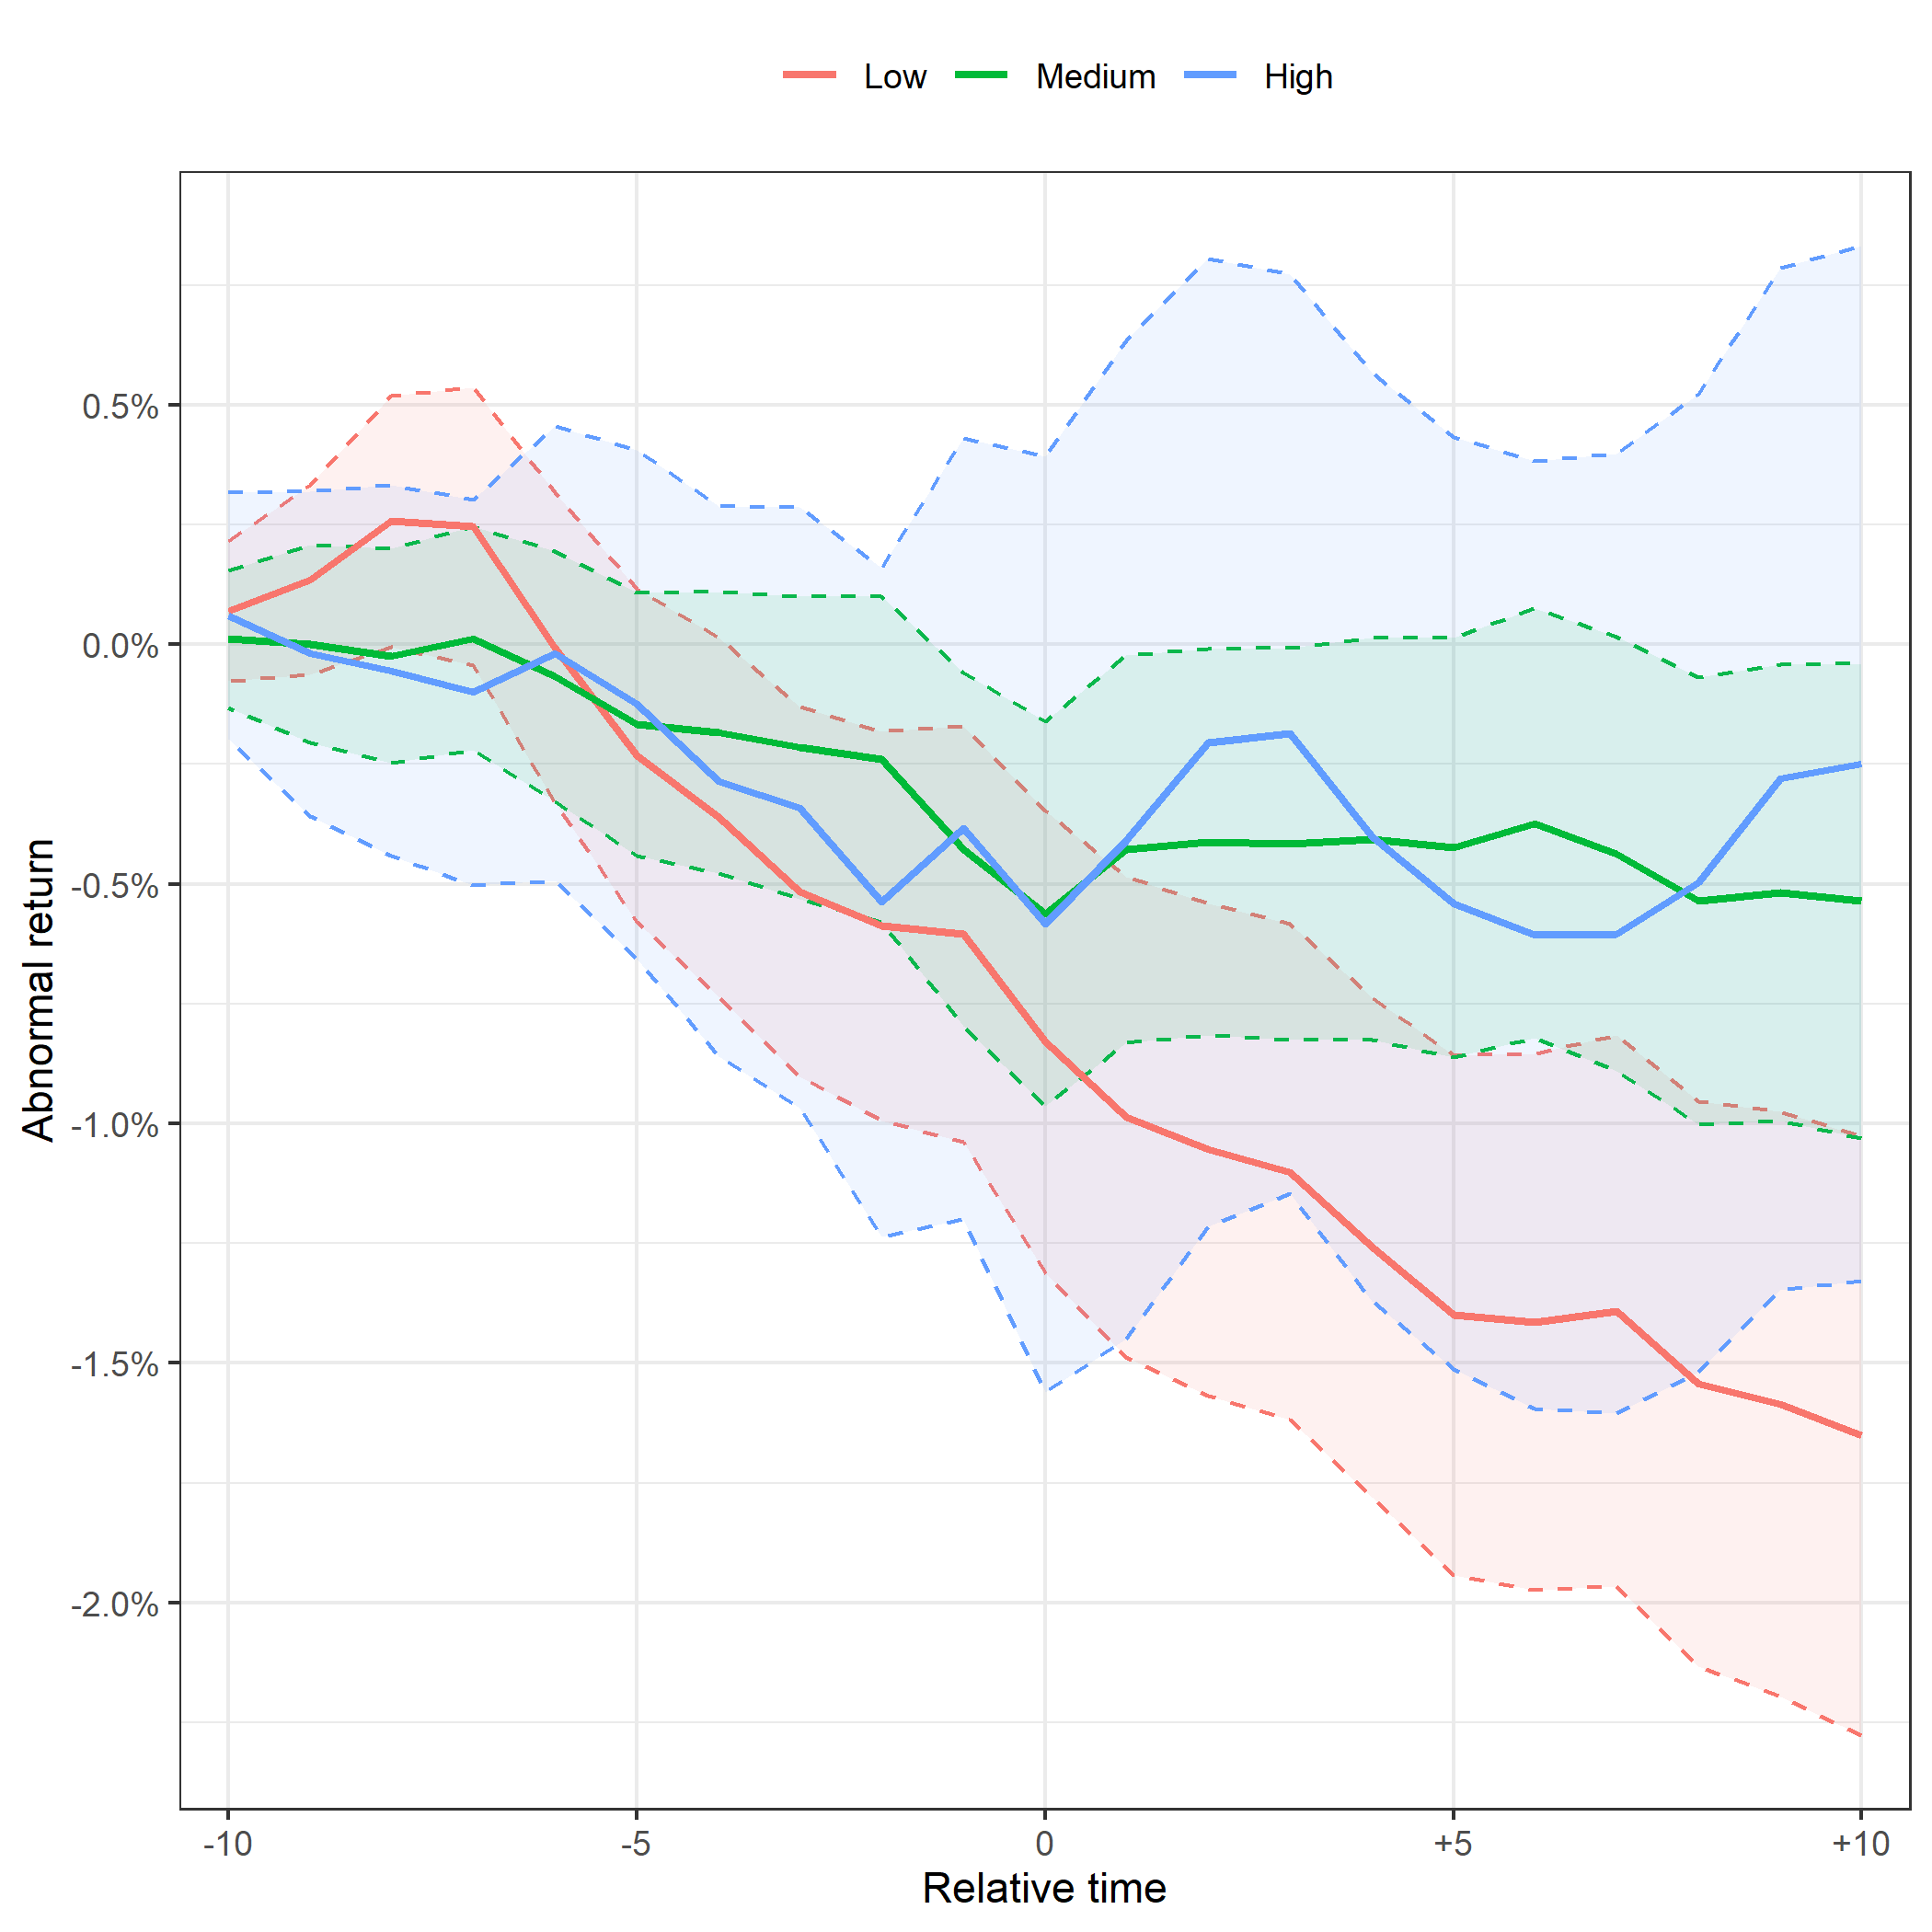
\includegraphics[scale=0.6]{Projekt/1.Figures analysis/ST_negative_ESG.png}
     \caption*{\footnotesize The figure illustrates the CAAR of firms, partitioned on ESG risk, 21 days around the event date (t = 0) after a negative event, along with $95\%$ confidence intervals. The outcome for the low-risk group is based on 504 events, 811 events for medium-risk, and 289 events for high-risk. Low-risk companies are penalized the most with a significant CAAR of $-1.65\%$ after a negative event. Medium risk companies are penalized at an average rate of $-0.54\%$ significant at $5\%$, whereas high-risk companies are not impacted significantly.     
     }
    \label{fig:ST_neg_ESG}
\end{figure} 

The CAAR of the three groups exhibit dissimilar patters, suggesting that the overall findings of significant, negative abnormal returns from figure \ref{fig:ST_neg_news} do not apply uniformly across all risk types. Nonetheless, firms with low and medium risk profiles both experience significant negative abnormal returns up of to -1.65\% and -0.54\%, respectively. The groups are barely statistically different from one another, however the distinction in mean values do imply a discrepancy in investor reactions. On the other hand, the group of high-risk companies, which consists of only 289 observed events, exhibits a CAAR of -0.25\% and no significant relationship can be determined due to the wide confidence intervals

\noindent \textbf{SDG Pillars.} Examining the abnormal returns associated with news related to specific SDGs has the potential to enhance our understanding of which themes within corporate sustainability that investors prioritize. The CAAR for each SDG over the full event window are illustrated in figure \ref{fig:ST_neg_bar_all} in the appendix. Due to the limited number of observations for certain SDGs, the CAAR results are highly insignificant, as indicated by the wide confidence intervals. This is particularly relevant for SDG 4 and 9, where only 16 and 74 negative events are identified, respectively. 

\begin{figure} [h]
    \centering
    \caption{Five Pillars of SDGs: Negative News}
    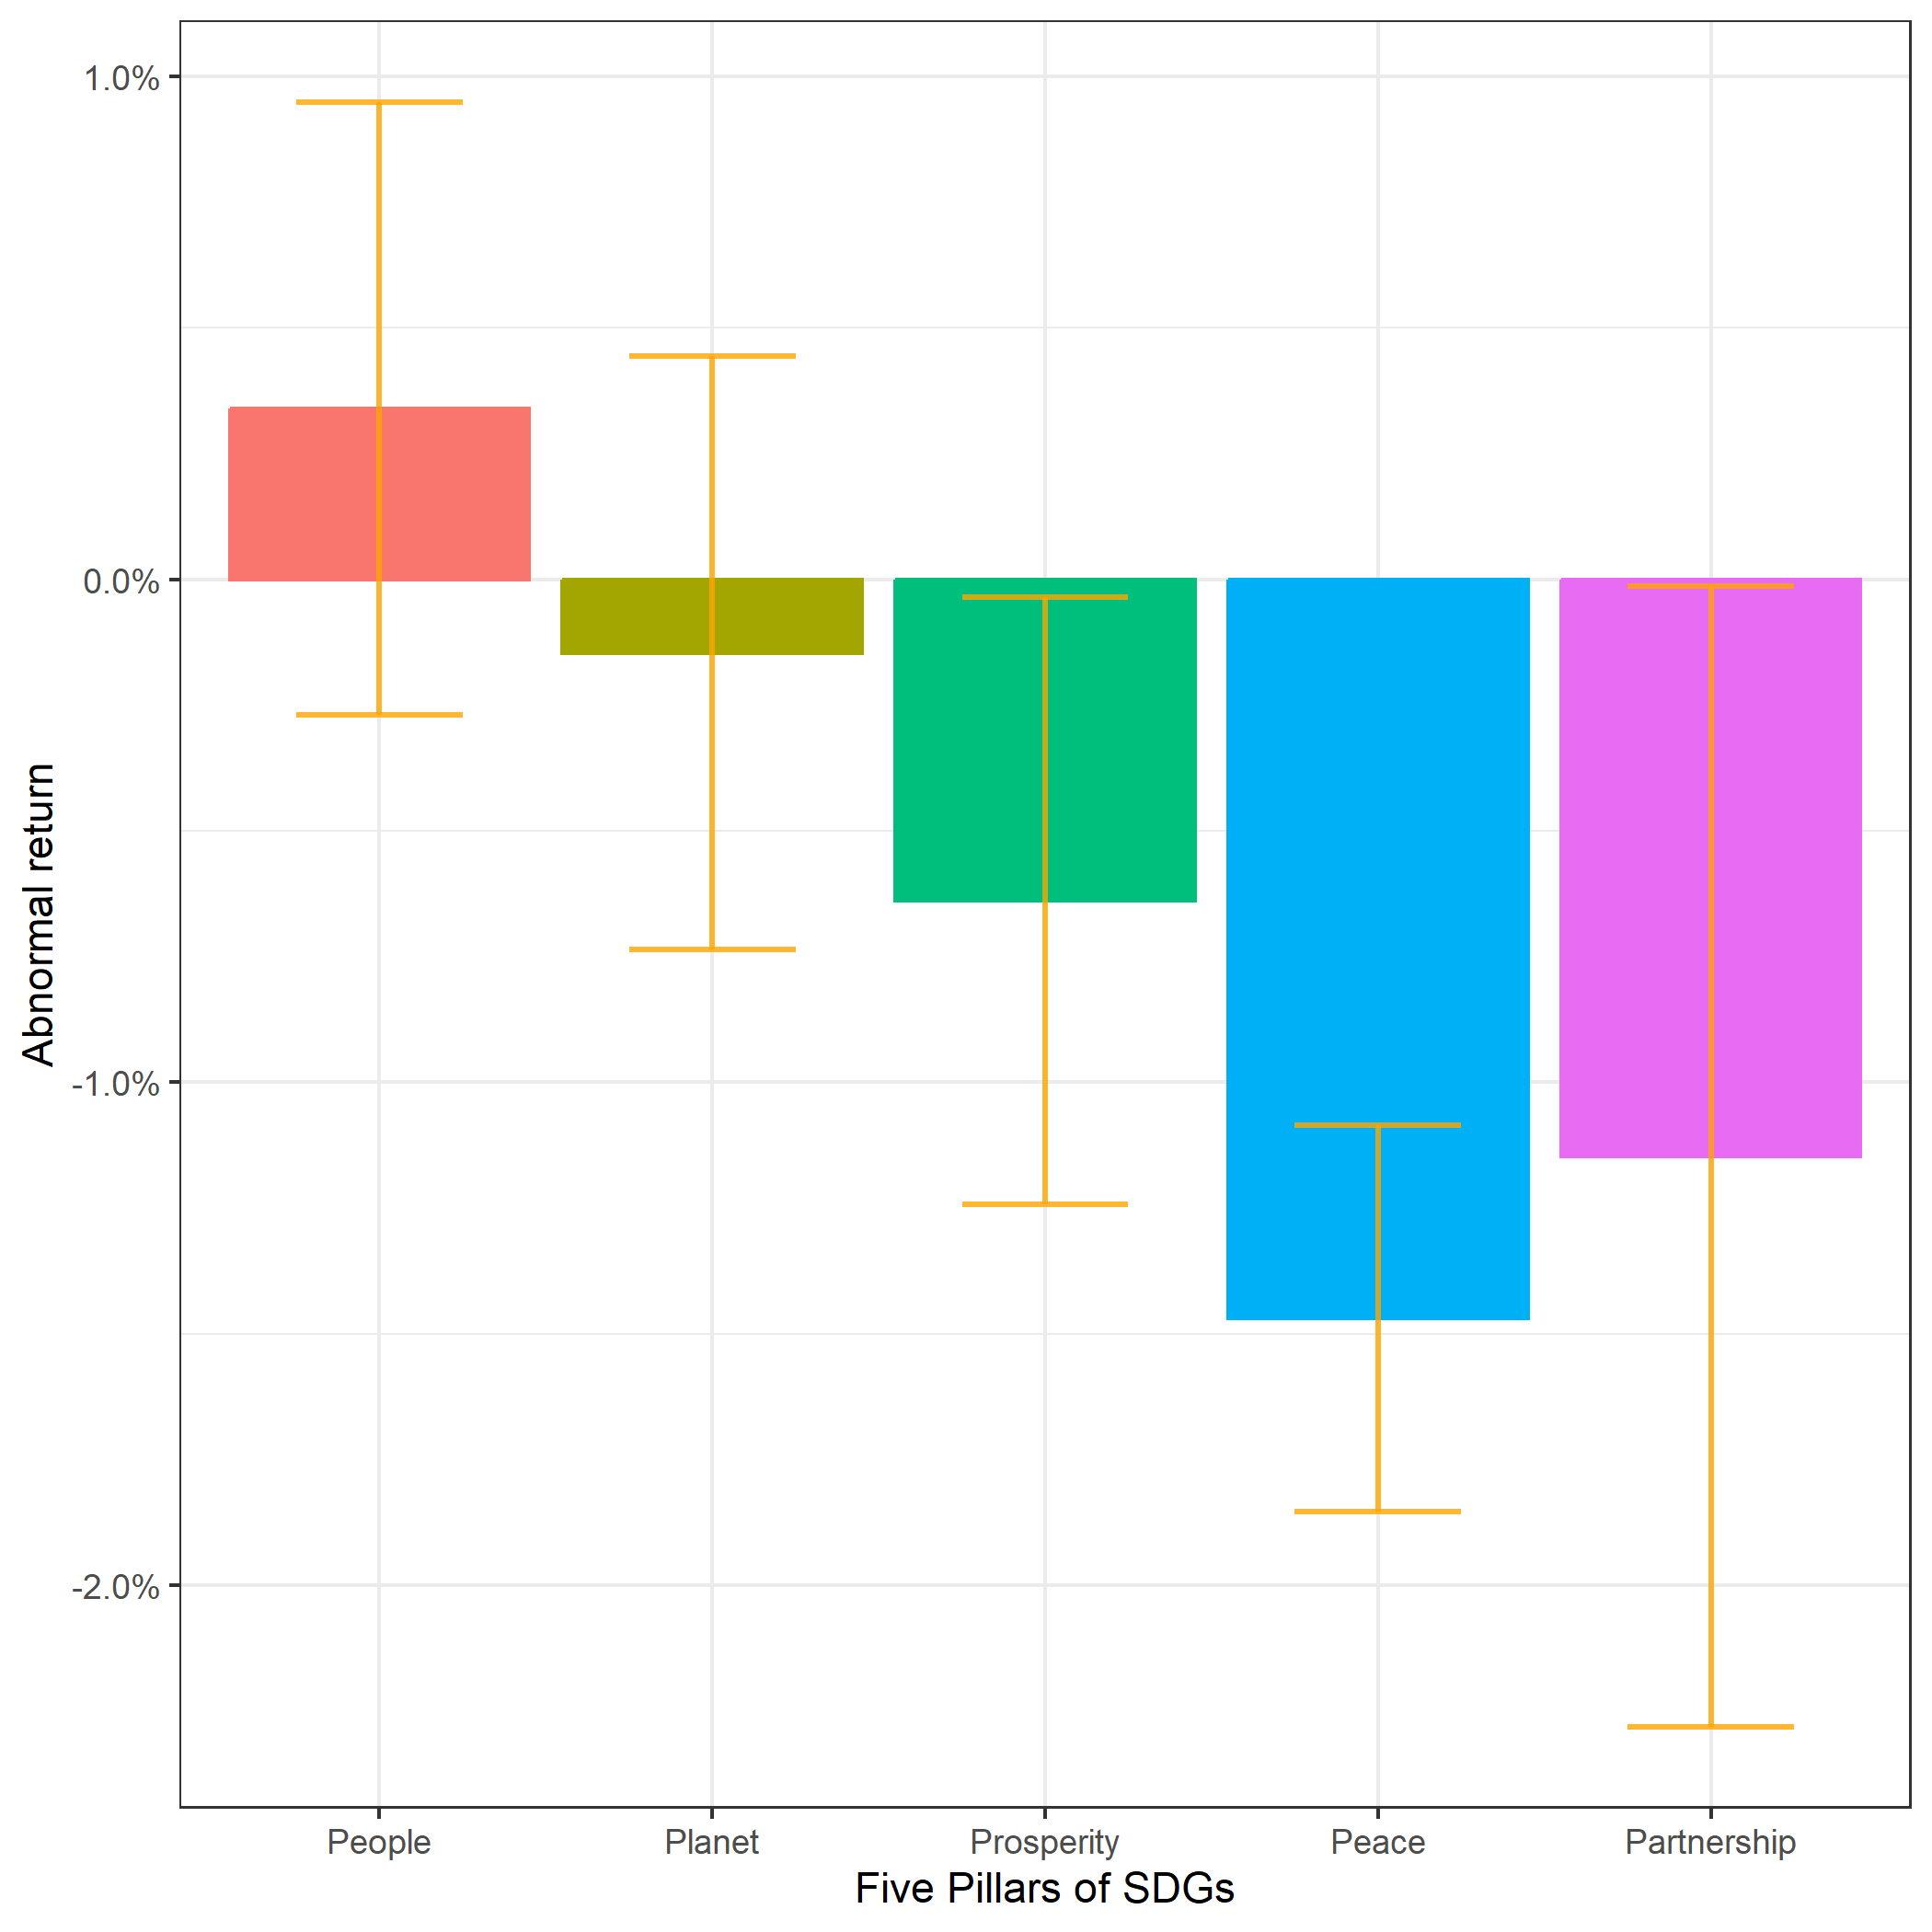
\includegraphics[scale=0.6]{Projekt/1.Figures analysis/ST_negative_sdg_bar_groups_0.png}
    \caption*{\footnotesize The figure illustrates the CAAR over the entire event window after negative events, along with 95\% confidence bands. The individual SDGs are grouped into themes by The Five Pillars of SDGs. The Pillars Planet, Peace, and Prosperity generates negative abnormal returns of $-0.70\%$, $-0.57\%$, and $-0.53\%$, respectively, with the two former being significant at a 5\% level. The outcomes are based on 1196, 1411, and 1087 events for the three Pillars, respectively. The People and Partnership Pillars generate positive abnormal returns of $0.48\%$ and $0.37\%$ from 1145 and 239 events, respectively. 
    }
    \label{fig:ST_neg_bar}
\end{figure}

To address this limitation, I adopt a categorization approach by grouping the SDGs into five themes commonly referred to as the "Five Pillars of SDGs"\footnote{https://unsdg.un.org/latest/videos/5ps-sdgs-people-planet-prosperity-peace-and-partnership}, which consist of People, Prosperity, Planet, Peace, and Partnership\footnote{The groups consist of the following SDGs: People (1,2,3,4,5), Prosperity (7,8,9,10,11), Planet (6,12,13,14,15), Peace (16), Partnership (17)}.
This approach enables a shift in focus from individual SDGs to broader sustainability themes, thereby allowing for a more comprehensive examination of the research questions. Figure \ref{fig:ST_neg_bar} illustrate the CAAR over the full event window for negative news related to the Five Pillars of SDGs.
The results show that the themes Planet, Prosperity, and Peace are associated with negative CAARs of -0.70\%, -0.53\%, and -0.57\%, respectively, whereas People and Partnerships, are associated with insignificantly positive abnormal returns of 0.49\% and 0.37\%, respectively. Investors clearly have a preference for specific themes within sustainability. 

\subsubsection{Positive Pews}

\textbf{Overall SDGs}
According to figure \ref{fig:ST_pos_news}, investors react promptly to positive events, as abnormal returns are present on the event day, while the remaining days of the window are not associated with a significant reaction from shareholders. The CAAR revolves around 0\% as well with a slight top on the event date. Although insignificant, a slightly positive reaction is present, however the average effect reverts to zero throughout the event window. 

\begin{figure} [h]
     \centering
     \begin{minipage}[t]{0.49\textwidth}
         \centering
    \caption{Positive News: AAR and CAAR \\}
    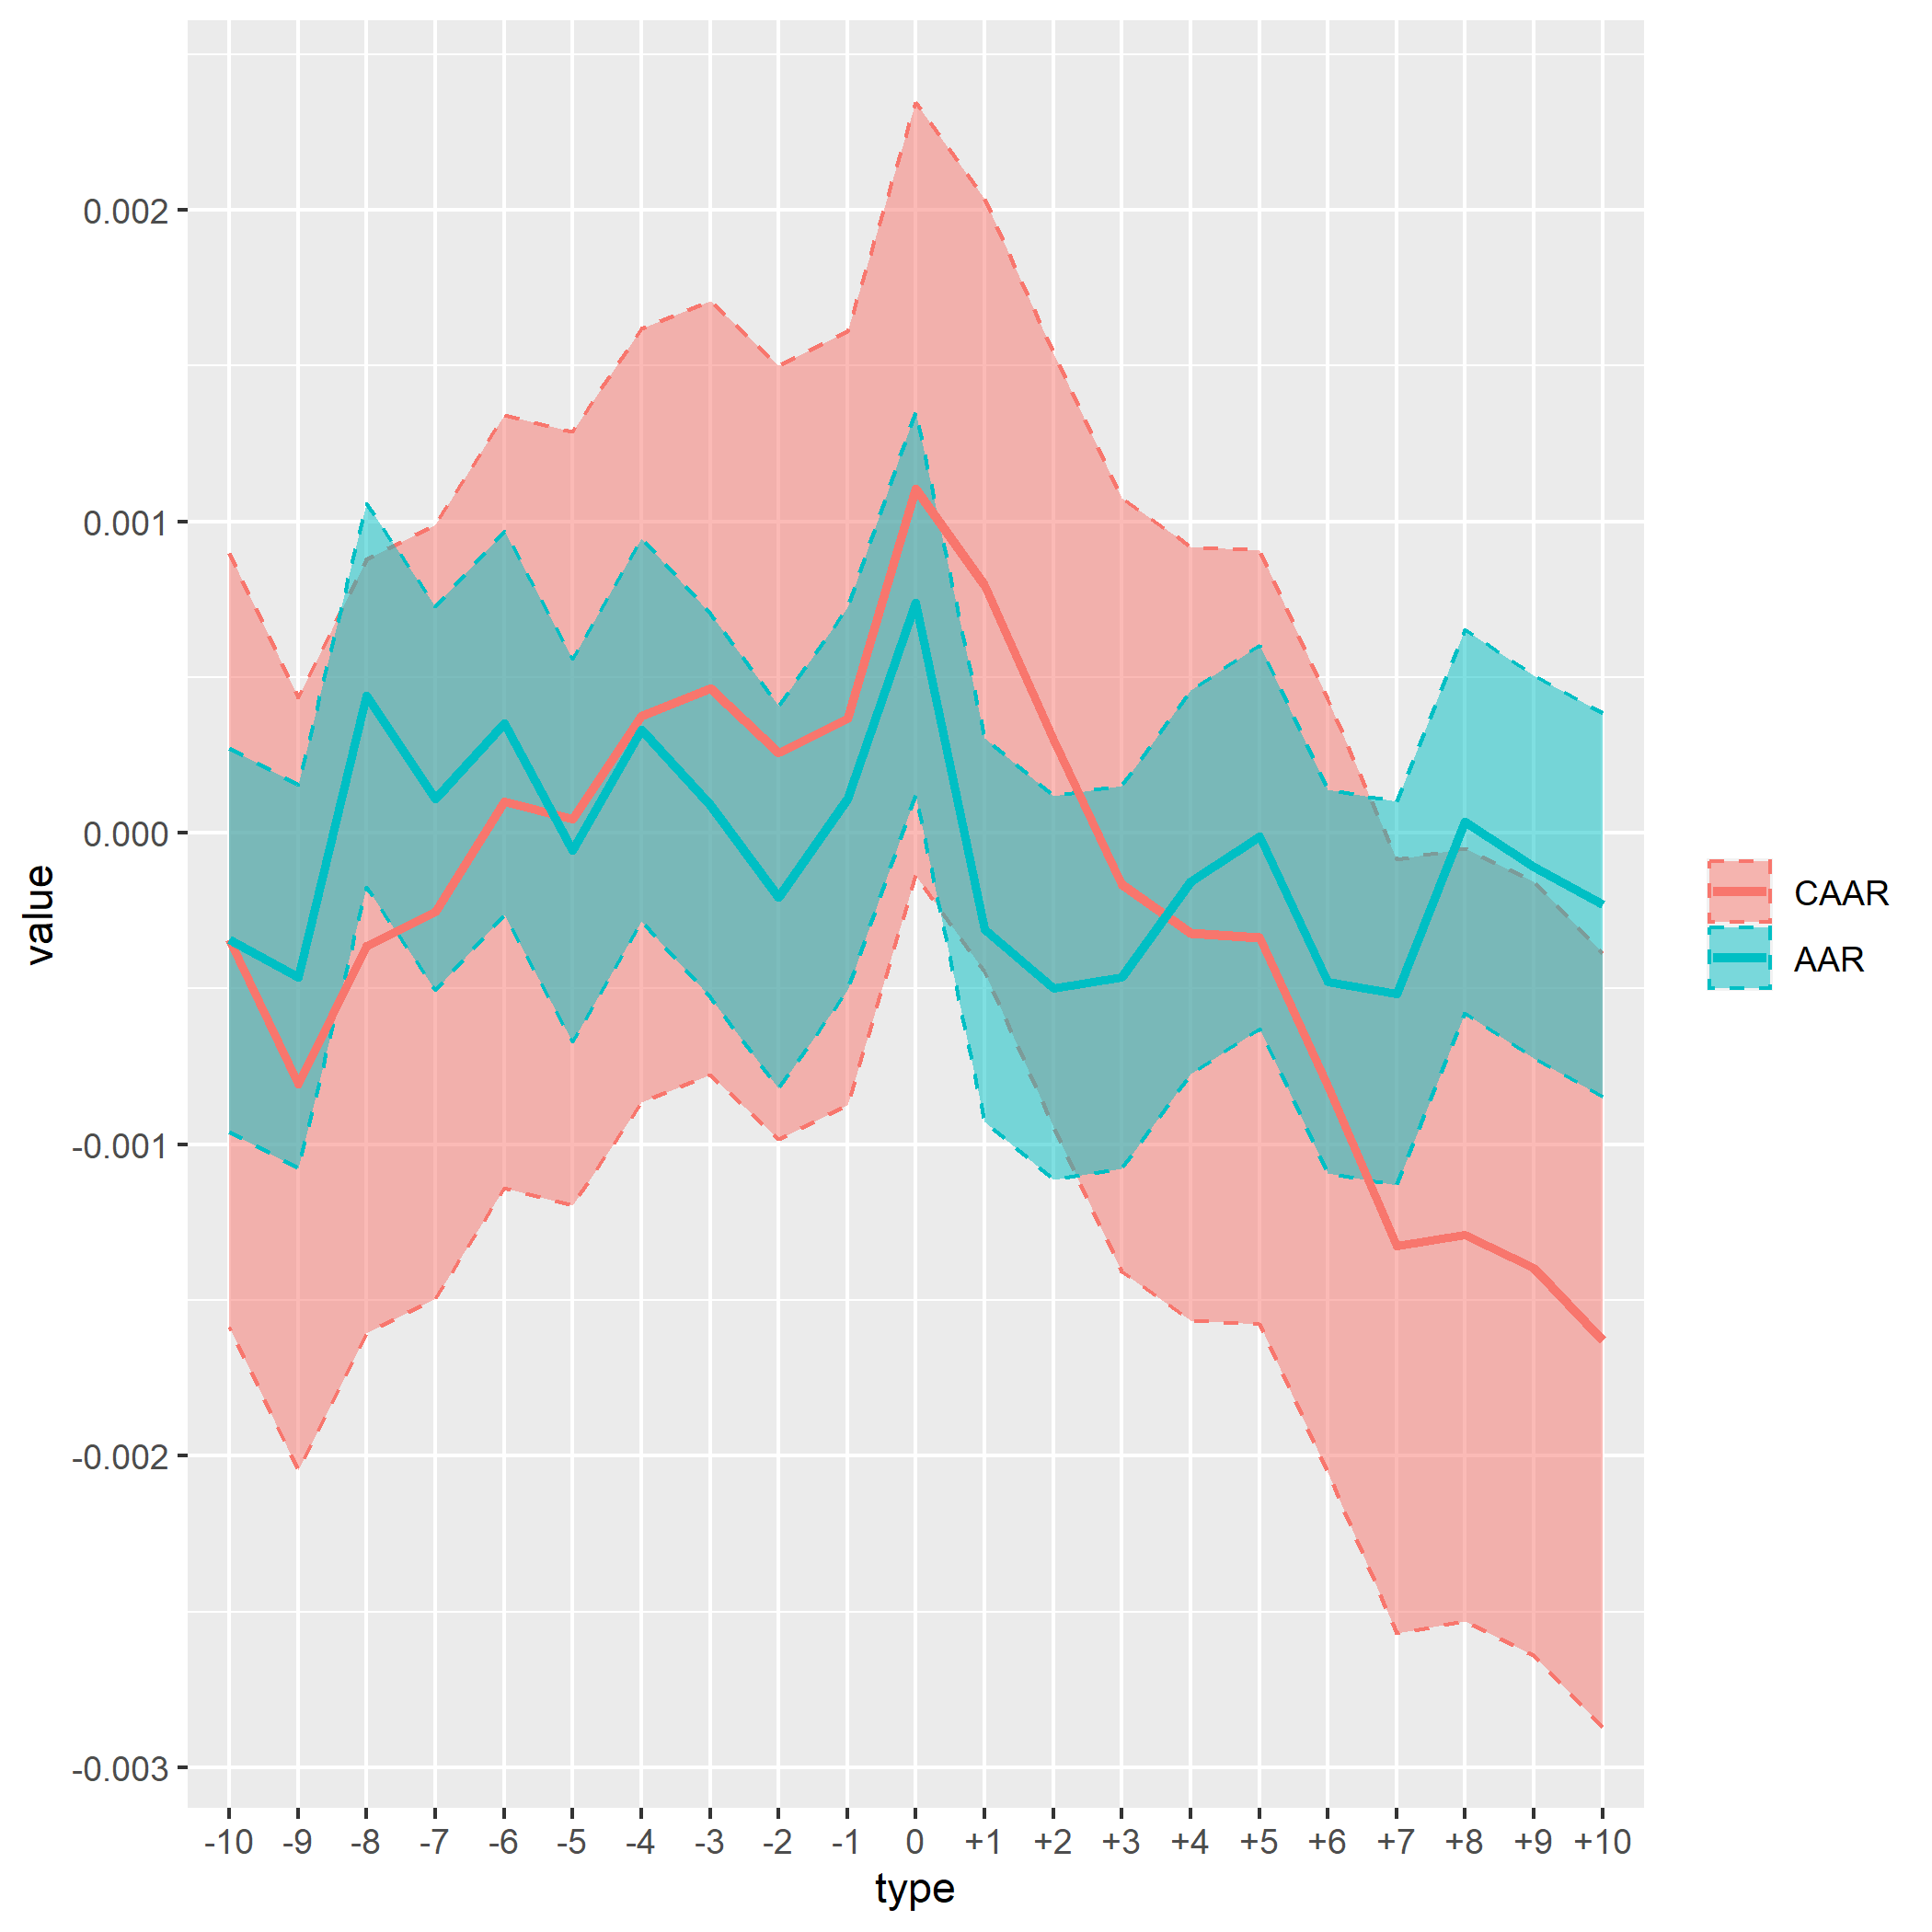
\includegraphics[width=\textwidth]{Projekt/1.Figures analysis/ST_positive_all_CI.png}
    \caption*{\footnotesize The figure illustrates the AAR and CAAR around the event date (t = 0) after positive events, along with 95\% confidence intervals and the relative number of events on a given day relative to the event date (rhs). The outcome is based on N = 10,420 events. The investors react significantly positive on the event date with an AAR of $0.05\%$. However, the impact is insignificant over the full event window with a CAAR of $-0.02\%$.\\}
     \label{fig:ST_pos_news}
     \end{minipage}
     \hfill
     \begin{minipage}[t]{0.49\textwidth}
       \centering
    \caption{CAAR Partitioned on ESG Risk Ratings: Positive News}
    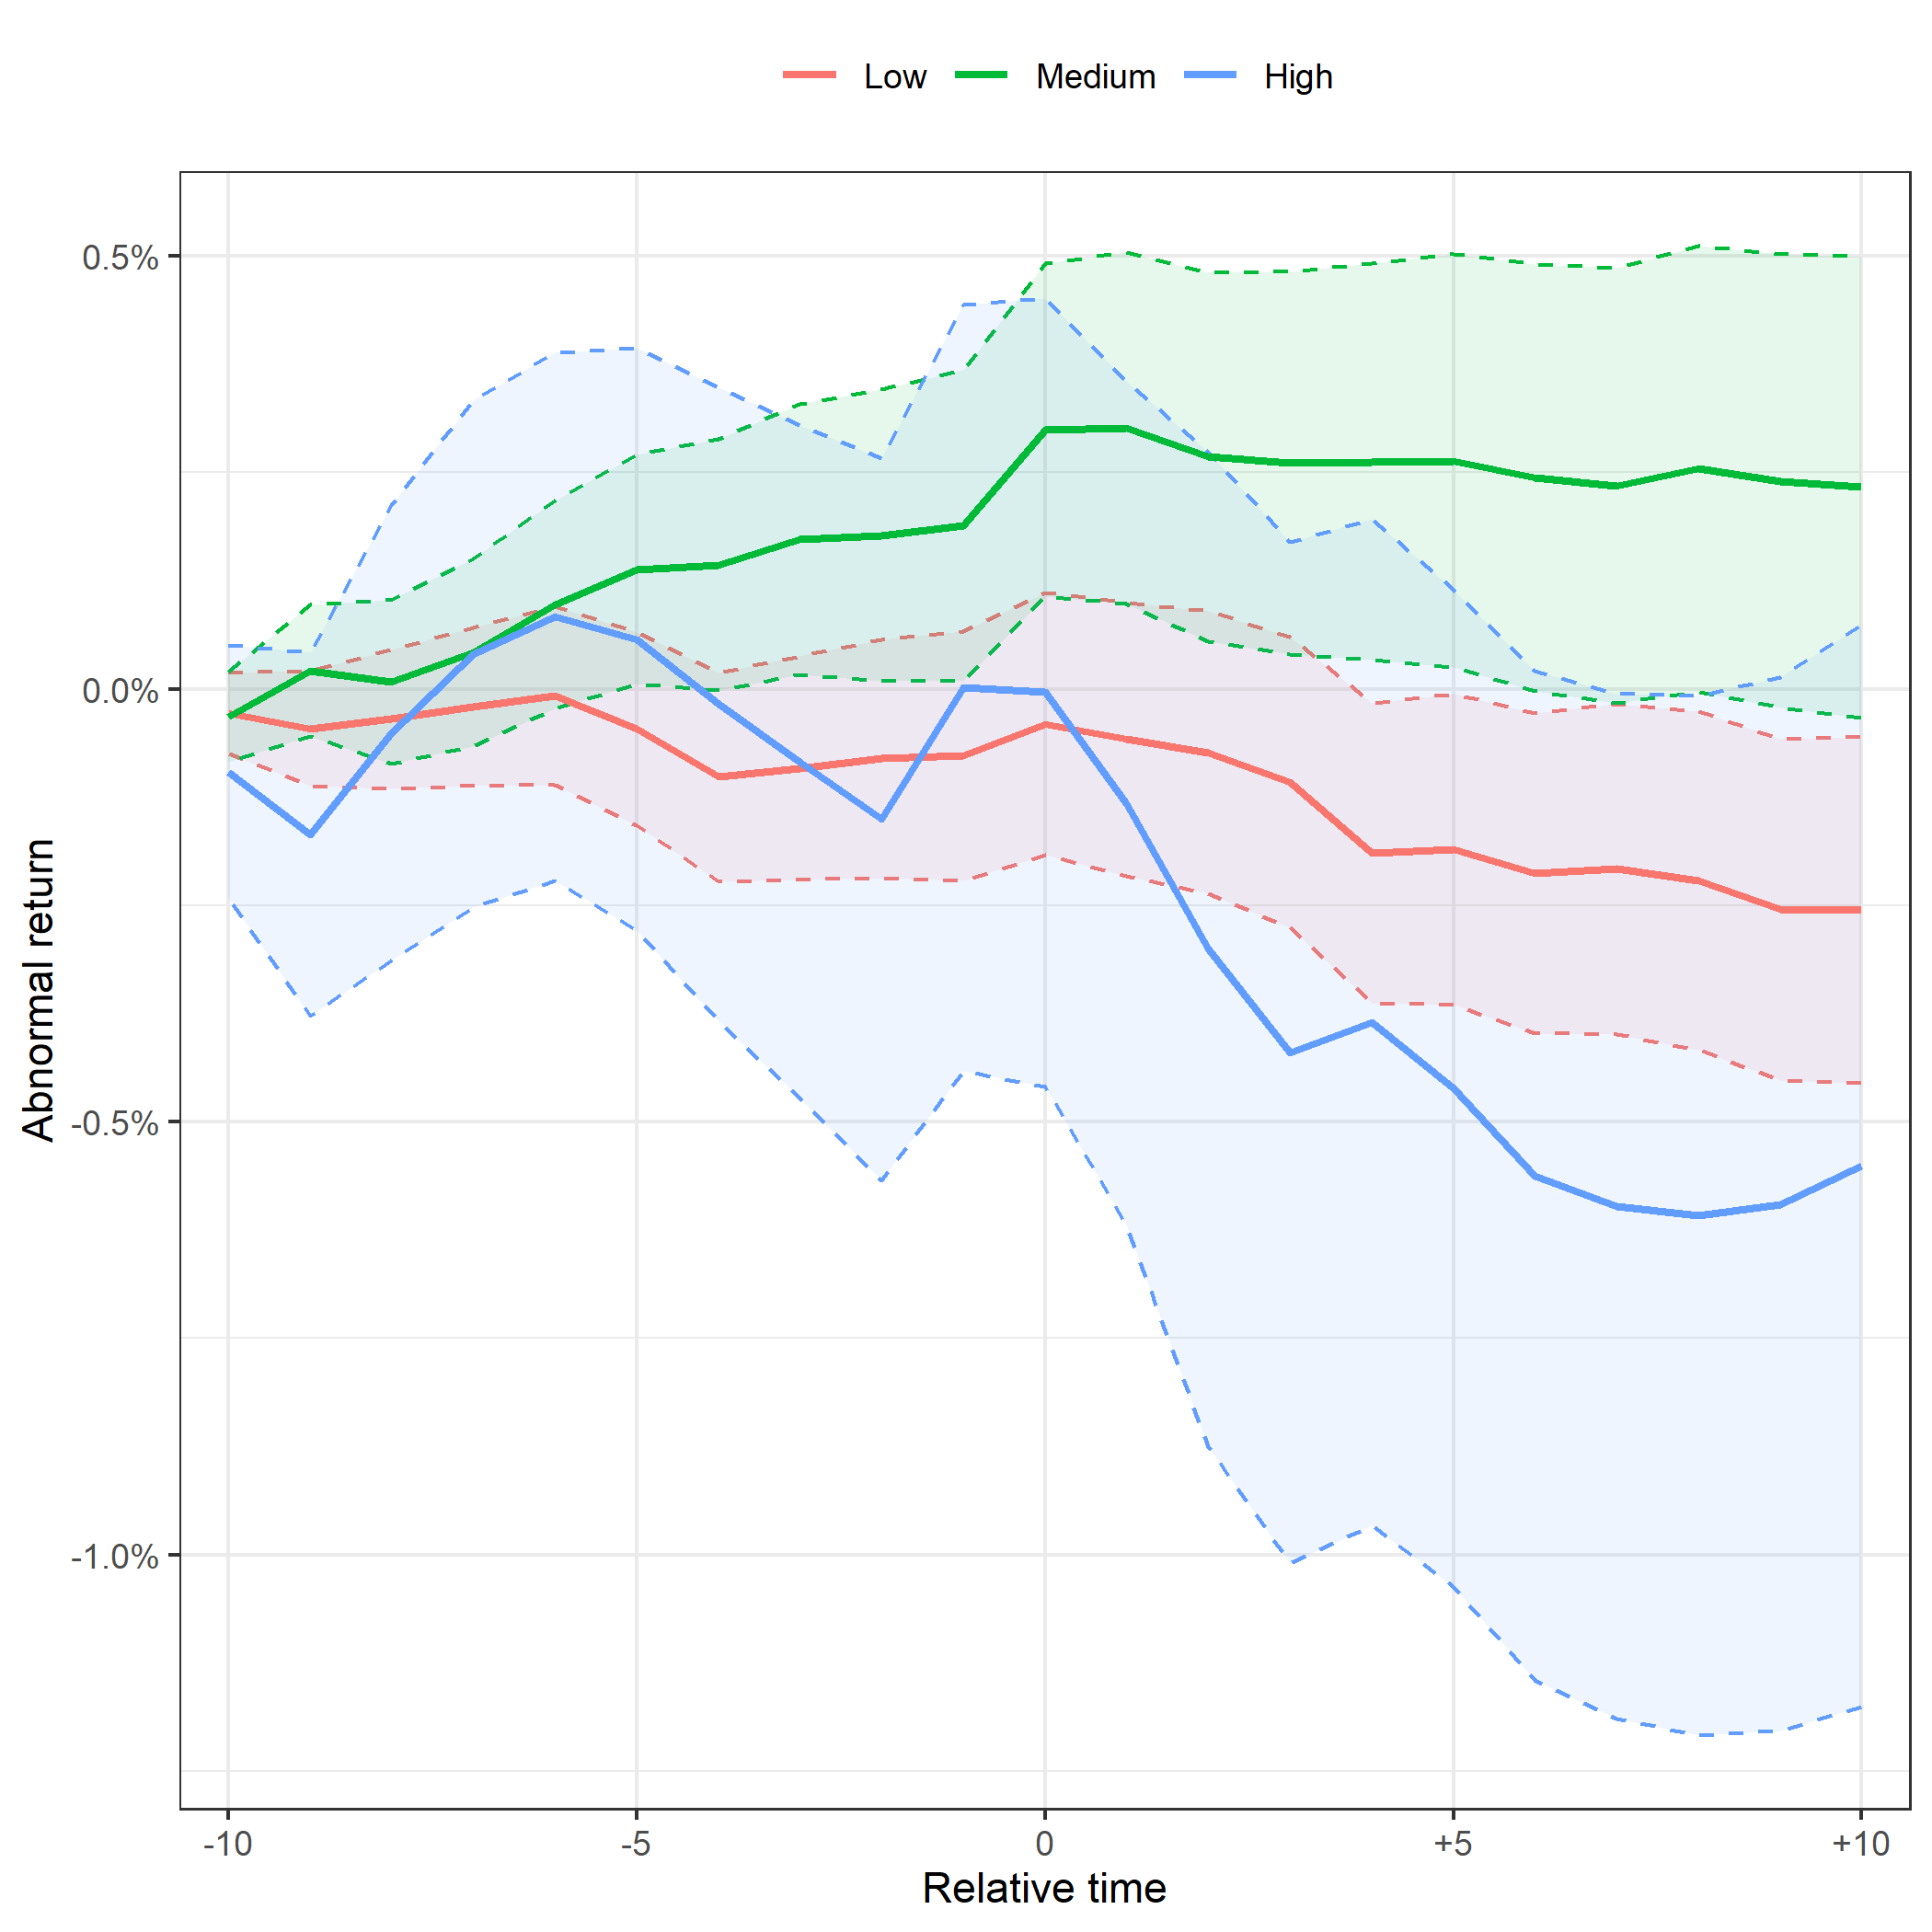
\includegraphics[width=\textwidth]{Projekt/1.Figures analysis/ST_positive_ESG.png}
    \caption*{\footnotesize The figure illustrates the CAAR of firms, partitioned on ESG risk, 21 days around a positive event, along with $95\%$ confidence intervals. The outcome for the low-risk group is based on 4,989 events, 4760 events for medium-risk, and 627 events for high-risk. High-risk companies are impacted the most, on average, with a CAAR of -0.53. However, this average comes with high uncertainty and is not significantly different from zero at a 5\% level. Medium- and low risk companies face reactions corresponding to CAAR values of $0.24\%$ and $-0.23\%$, respectively, both significant on at least a 5\% level.}
    \label{fig:ST_pos_ESG}
     \end{minipage}
        
\end{figure}

\noindent \textbf{Partition on ESG risk.} Average results alone do not fully capture the narrative, as figure \ref{fig:ST_pos_ESG} highlights a notable distinction between firms with low and medium ESG risk profiles. Shareholders demonstrate a pessimistic reaction, with a significantly negative CAAR of -0.25\%, when low ESG risk firms engage in positive interactions with SDGs. 
High ESG risk firms, on the other hand, experience negative abnormal returns of approximately -0.5\%, although the average result comes with high uncertainty. In contrast, firms with a medium risk rating enjoy a significant and positive CAAR at $0.25\%$ over the entire  window. 

\noindent \textbf{SDG Pillars}
The tendencies of insignificance are further emphasized by the abnormal returns across the Five Pillars of SDGs for positive events. In contrast to the issue of insufficient observations in the case of negative events, the underlying uncertainty emerges from the seemingly random shareholder reaction to positive events in general, as indicated by the aggregate overview in figure \ref{fig:ST_pos_bar}. 
Only SDGs 4, 8, and 10, demonstrates significantly abnormal returns over the full window as per figure \ref{fig:ST_pos_bar_all} in the appendix. While People, Peace, and Partnership exhibit negative abnormal returns, Planet and Prosperity display positive abnormal returns. However, none of these results reach statistical significance at a 5\% level.   


Overall, the short term empirical results demonstrate insights into the relationship between SDG events and corporate performance. Negative events are associated with an average penalty of -0.72\% from shareholders, whereas shareholders does not react to positive events. When considering ESG risk characteristics, I find that low-risk firms are penalized the most from negative events. Interestingly, medium risk-firms are rewarded for positive events, while low-risk firms face are penalized. Accounting for SDG themes reveals that shareholders react significantly negative to adverse news related to prosperity, peace, and partnerships, whereas no significant reaction is observed from positive news. 

\begin{figure} [H]
    \centering
    \caption{Five Pillars of SDG: Positive news}
    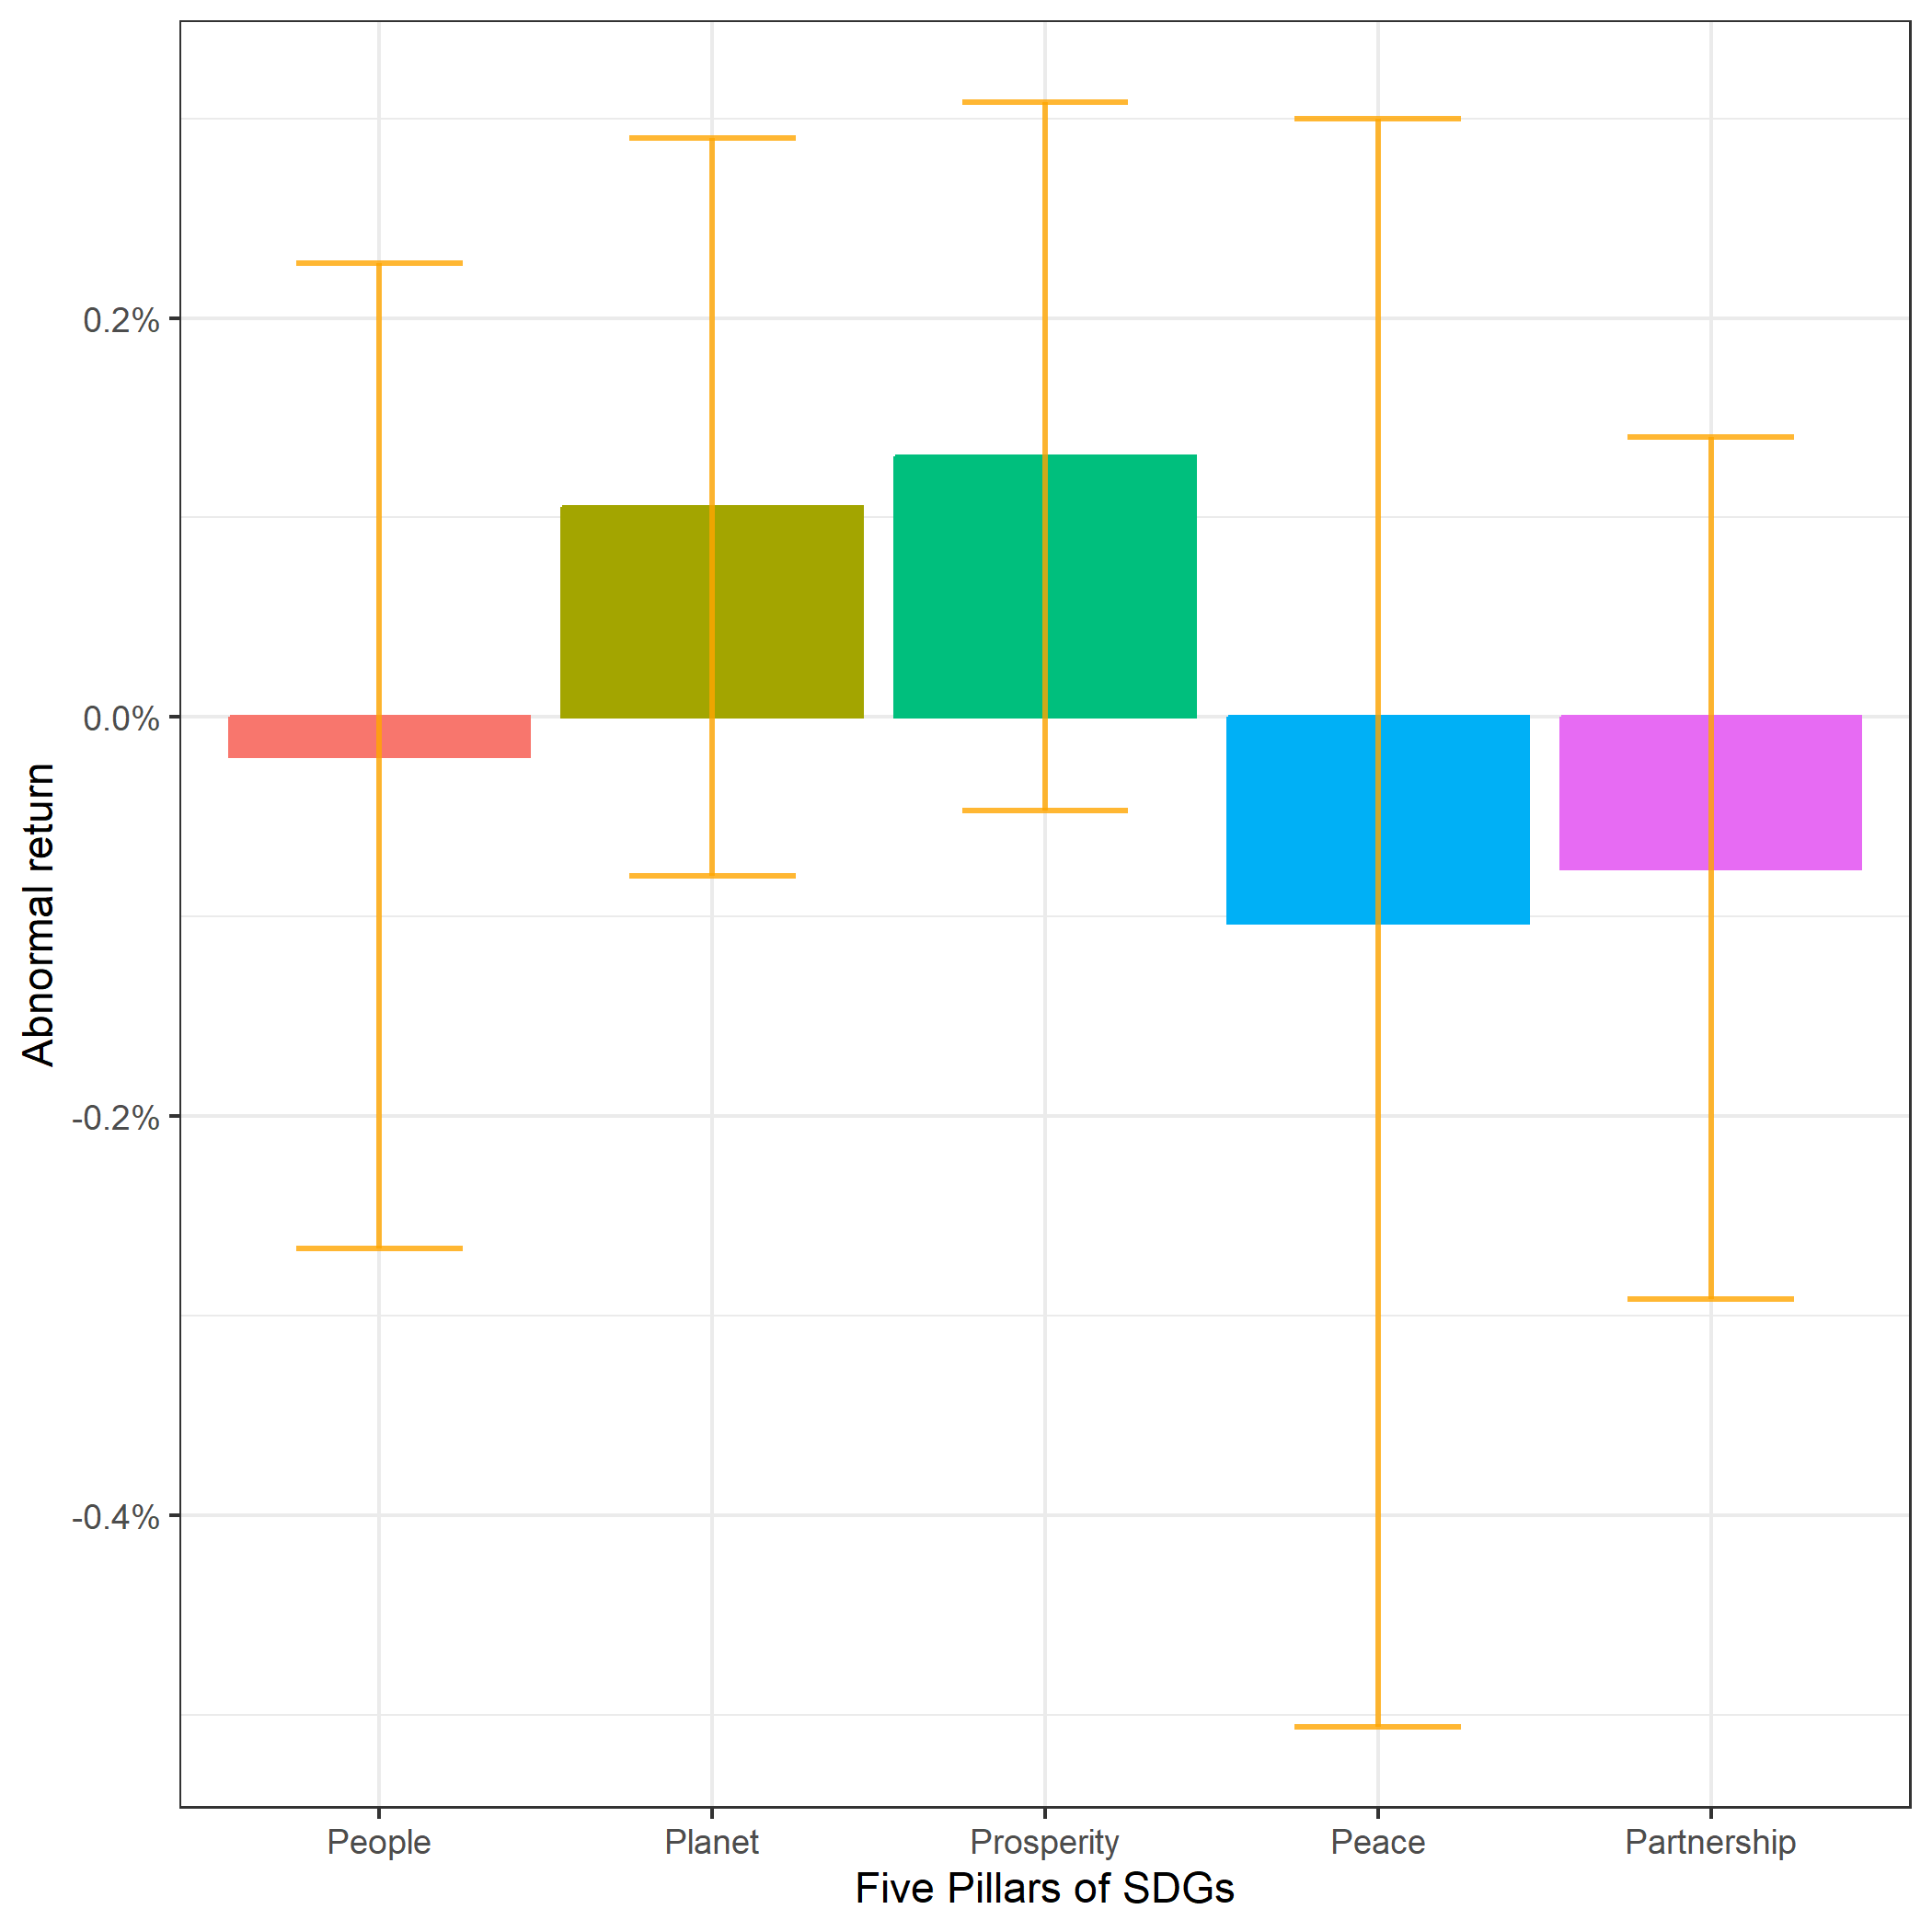
\includegraphics[scale=0.6]{Projekt/1.Figures analysis/ST_positive_sdg_bar_groups_0.png}
    \caption*{\footnotesize 
    The figure illustrates the CAAR over the entire event window after negative events, along with 95\% confidence bands. The individual SDGs are grouped into themes by The Five Pillars of SDGs. The Pillars Planet and Prosperity generates positive, but insignificant, abnormal returns of $0.1\%$ and $0.12\%$, respectively. The outcomes are based on xx and xx events, respectively. The People and Partnership Pillars generate positive abnormal returns of $0.48\%$ and $0.37\%$ from 1395 and 234 events, respectively. 
    
    The figure illustrates the CAAR on $t = 10$ (full period) from positive news. The error bars represent the 95\% confidence intervals of the CAAR.}
    \label{fig:ST_pos_bar}
\end{figure}

\subsection{Long Term Abnormal Returns} \label{sec: long_term_portfolio}

In contrast to the short-term methodology, where all abnormal returns are averaged to a single event day, the long-term portfolios are rebalanced on a monthly basis, and they include all firms that have experienced an event within the previous T [1,4,8,12] months. The performance of these portfolios is evaluated in accordance with the Calendar Time Portfolio approach, and White heteroskedastic-robust standard errors are applied to account for potential heteroskedasticity. Any evidence of autocorrelation in the models' residuals has been rejected by a Breusch-Godfrey test of first-order. Furthermore, the appendix provides all necessary regression statistics, including coefficient estimates, R-squared values, and standard errors for the significant models, for further reference and analysis.

Overall, the factor models demonstrate a strong ability to explain the risk exposure and excess returns of the portfolios, with R-squared coefficients ranging from 85\% to 98\% for the ordinary portfolios. The portfolios that hold the least amount of firms generally has the lowest r-squared, which seems to be a result of increased idiosyncratic variance. To maintain a sufficient number of observations in the portfolios, the analysis does not measure the performance from categorizing events into specific SDG themes. 

\subsubsection{Negative News}

The abnormal returns of the individual portfolios are captured by the intercept (alpha) estimated from the Fama-French regressions, as illustrated in table \ref{tab: FF5_neg_ESG} along with the corresponding t-statistics. The table includes an "Overall" column, which represents the alpha of the portfolio consisting of all firms that have experienced a negative event in a given calendar month. Additionally, there are three columns representing firms categorized based on their ESG risk rating. Each section in the table corresponds to a different portfolio holding period, denoted by "$T = x$" above each horizontal line.

Overall, the results reveal that negative events lead to negative alphas across all holding periods, which in part illustrates the effectiveness of the event selection methodology. The alphas are significantly negative, with values of -0.84\% at a 1\% level and -0.36\% at a 5\% level for holding periods of T = 1 and T = 4 months, respectively. However, as the holding period increases beyond four months, the alphas approach zero and become statistically insignificant. This finding supports the idea of market efficiency over longer time horizons. It is worth noting that portfolios with longer holding periods include more firms in each rebalancing, which tends to align the portfolio returns with the overall market return. 

\setlength{\tabcolsep}{15pt}
\begin{table}[h]
\small
\centering
\caption{Fama-French five-factor model alpha from negative news split on ESG risk} 
\begin{tabular}{ccccccc}
\hline \hline \\ 
 &     & Overall &    Low  &  Medium  &  High &  \\    \cline{3-6} 
& &  \multicolumn{4}{c}{ T = 1} & \\ \cline{2-6}
& Alpha    & -0.84^{***} & -0.64^{**}  & -0.61  & -2.21 &  \\ 
& t-value   & -3.13 & -1.88 & -1.35  & -1.43 &  \\
& &  \multicolumn{4}{c}{ T = 4} & \\ \cline{2-6}
& Alpha    & -0.36^{**} & -0.23  & -0.33  &  -0.84 & \\
& t-value &   -2.29 & -1.06 & -1.28  & -1.23 & \\
& &  \multicolumn{4}{c}{ T = 8} & \\ \cline{2-6}
& Alpha     & -0.15 & -0.01   & -0.28  & -0.27 &  \\
& t-value &   -1.21 & -0.08  & -1.35 & -0.51 &  \\
& &  \multicolumn{4}{c}{ T = 12} & \\ \cline{2-6}
& Alpha     & -0.08 & -0.09  & -0.19  & -0.25 &  \\
& t-value &    -0.86 & -0.62  & -1.23 & -0.48 &  \\
\hline \hline
 \multicolumn{7}{l}{ \footnotesize $^* \; p\; <\; 0.1$, $ ^{**} \; p\; <\; 0.05$, $ ^{***} \; p\; <\; 0.01$  } \\
 \multicolumn{7}{p{12cm}}{ \footnotesize Alpha is the WLS-regression intercept (in \%) of the Fama-French 5-factor model, displayed along with the corresponding White heteroskedasticity-robust t-value. N is the average amount of firms included in the portfolio each month, and T is the portfolio holding period. The threshold for event firms to be included in the portfolio is either 1,2 or 3 "SD" (standard deviations) larger than the mean.} \\ 
 \hline
\end{tabular}
\label{tab: FF5_neg_ESG}
\end{table}


With a partition on ESG-risk, the negative alphas persist across all categories,  providing further confirmation of the initial inference. 

Low- and medium-risk portfolios generate alphas of approximate even magnitude at $-0.64\%$ and $-0.61\%$, respectively, with the former being significant at 5\%. On the other hand, portfolios with high ESG risk show considerably larger negative alphas, with values of -2.3\% and -0.84\% for holding periods of one and four months, respectively. For portfolios consisting of high-risk firms, the monthly rebalancing results in a small number of constituents due to the limited sample size of high-risk firms. As a result, the portfolios are more exposed to idiosyncrasies, which compromise the ability of the factor models to explain the portfolio returns through the systematic risk factors. Consequently, this implicates that the r-squared of the regressions become very low at 0.4 and 0.53, indicating that more of the variation in the portfolio returns is attributed to the error terms rather than the systematic risk factors. 

Across all subsets, the relation between negative news and returns are most severe within 1-4 months after an event has occurred.

\subsubsection{Positive News}

The impact of positive events on long-term market values is illustrated in table \ref{tab: FF5_pos}. The table follows the same format as table \ref{tab: FF5_neg_ESG}. Without partitioning on ESG risk, positive events have no significant impact on returns over any of the holding periods. The performance is most negative when using a brief holding period of $T=1$, with an alpha of of -0.26\%, which appears in line with the short term relation. Such results are indicative of a pessimistic short-to-medium term investor reaction to general positive news. However, since the alphas are not statistically significant in any of the cases, the overall inference is that there is no significant relationship between positive news and stock returns. This suggests that the portfolio returns resemble those of a well-diversified portfolio, which closely aligns with the returns of the overall market portfolio. This result is expected if we assume that positive news is generally perceived as irrelevant by investors in the long term.

\setlength{\tabcolsep}{15pt}
\begin{table}[h]
\small
\centering
\caption{FF-5 model alpha from positive news split on ESG risk} 
\begin{tabular}{ccccccc}
\hline \hline \\  
 &     & Overall  &    Low  &  Medium  &  High  &  \\ \cline{3-6} 
& & \multicolumn{4}{c}{ T = 1} & \\ \cline{2-6}
& Alpha   & -0.26 & -0.04  & -0.41  & -0.59 &  \\
& t-value & -1.03 & -0.12 & -1.47  & -0.47 & \\
& &  \multicolumn{4}{c}{ T = 4} & \\ \cline{2-6}
& Alpha   & -0.04 & -0.22  & -0.18  &  0.90 & \\
& t-value & -0.26 & -1.15 & -0.91  & 1.15 & \\
& &  \multicolumn{4}{c}{ T = 8} & \\ \cline{2-6}
& Alpha   & 0.01 & -0.23   & 0.03  & 1.06 &  \\
& t-value & 0.05 & 1.64  & 0.26 & 1.65 & \\
&  &  \multicolumn{4}{c}{ T = 12} & \\ \cline{2-6}
& Alpha   & 0.05 & -0.14  & 0.02  & $0.97^{*}$ &  \\
& t-value & 0.76 & -1.11  & 0.19 & 1.72 & \\
\hline \hline
 \multicolumn{7}{l}{ \footnotesize $^* \; p\; <\; 0.1$, $ ^{**} \; p\; <\; 0.05$, $ ^{***} \; p\; <\; 0.01$  } \\
 \multicolumn{7}{p{12cm}}{ \footnotesize Alpha is the WLS-regression intercept (in \%) of the Fama-French 5-factor model, displayed along with the corresponding White heteroskedasticity-robust t-values. T is the portfolio holding period. The threshold for event firms to be included in the portfolio is 1 standard deviation from the mean.}  \\ 
\end{tabular}
\label{tab: FF5_pos_ESG}
\end{table}

For the low ESG risk portfolio with a holding period of one month, the alpha is practically zero at -0.04\%, indicating no significant abnormal returns from positive events. The medium ESG risk portfolio exhibits a slightly higher alpha of -0.41\%, however still not statistically significant. Surprisingly, the high ESG risk portfolio shows significant positive alphas for holding periods longer than four month. With T = 1 the abnormal returns are negative - on par with the short term results. The fluctuating trend of the alphas along with low r-squared in the range of 0.48\% to 0.63\% indicate that the results from the high-risk portfolios are unreliable. 

In summary, the combined findings from short and long-term empirical results reveal that investor tend to react adverse to negative news, whether it is an immediate reaction or a lasting impact over several months. This negative reaction is most pronounced when it comes to companies with lower ESG risk levels. On the other hand, positive news does not appear to generate a significant response from investors. In the next sections, I will examine the validity of these results by testing parts of the assumptions. 